{\bfseries El tema 4 por fin introduce la inteligencia artificial, comenzando por el aprendizaje supervisado}

\section{Introducción al machine learning} 
El machine learning, o aprendizaje automático, es una rama de la inteligencia artificial que se centra en el desarrollo de algoritmos y técnicas que permiten a las computadoras aprender de y hacer predicciones sobre datos. A través del uso de modelos matemáticos y estadísticos, las máquinas pueden identificar patrones y tomar decisiones con mínima intervención humana.

Todo el proceso tiene \textbf{5 pasos principales}:
\begin{enumerate}
    \item Recoger Datos.
    \item Preprocesamiento de datos
    \item Elegir el mejor modelo.
    \item Entrenar y ajustar los parámetros del modelo.
    \item Ver si los resultados del modelo predicen correctamente nuevos datos.
\end{enumerate}

\subsection{Recoger Datos}

Los datos se pueden obtener de muchas maneras: Mediante web scraping, desde una API o base de datos\dots
Pero como vamos a realizar aprendizaje supervisado necesitamos \textbf{datos etiquetados}.

\renewcommand{\arraystretch}{1.5} % Espaciado entre filas
\newcolumntype{C}[1]{>{\centering\arraybackslash}m{#1}} % Columnas centradas

\begin{table}[h!]
\centering
\setlength{\arrayrulewidth}{0.3mm} % Grosor de las líneas de la tabla
\setlength{\tabcolsep}{5pt} % Espaciado horizontal en celdas

\begin{tabular}{|C{1cm}|C{1cm}|C{1cm}|C{1cm}|C{1cm}|C{1cm}|C{1cm}|C{1cm}|C{1cm}|C{1cm}|C{1cm}|}
\hline
\textbf{age} & \textbf{gender} & \textbf{height} & \textbf{weight} & \textbf{ap\_hi} & \textbf{ap\_lo} & \textbf{cholest} & \textbf{gluc} & \textbf{smoke} & \textbf{alco} & \textbf{cardio} \\
\hline
46.0 & F & 172 & 112 & 120 & 80 & 1 & 1 & 0 & 0 & YES \\
\hline
44.0 & M & 170 & 69 & 120 & 70 & 1 & 1 & 0 & 1 & NO \\
\hline
45.5 & M & 159 & 49 & 120 & 70 & 1 & 1 & 0 & 0 & NO \\
\hline
39.7 & F & 164 & 48 & 110 & 70 & 1 & 2 & 1 & 1 & YES \\
\hline
63.3 & F & 180 & 104 & 120 & 85 & 2 & 2 & 0 & 0 & NO \\
\hline
\end{tabular}
\caption{Ejemplo de datos etiquetados}
\label{tab:datos_etiquetados}
\end{table}

Por ejemplo en la tabla \ref{tab:datos_etiquetados} tenemos datos de pacientes y si han tenido un ataque al corazón o no. Los datos etiquetado se elegirán dependiendo de la variable que queramos predecir:

\[ \{ (x[i], y[i]) \mid x[i] \in \mathbb{R}^n,\ y[i] \in \{c_1, c_2, \dots, c_m\},\ i = 1, \dots, N \} \]

Todo esto con el objetivo de generar un modelo acorde a la fórmula: $ \hat{Y} = f\left(x, w\right) $ Siendo $x_n$ cada variable y $w$ los pesos de cada variable.

\subsection{Preprocesamiento de datos}

El preprocesamiento de datos es una etapa crítica en el proceso de machine learning, ya que los datos sin procesar pueden contener errores, valores atípicos o información redundante que puede afectar la precisión de los modelos. Algunas técnicas comunes de preprocesamiento de datos incluyen la limpieza de datos, la normalización de datos y la selección de características. A continuación se detallarán las técnicas de preprocesamiento a usar.

\subsubsection{Missing Values}
Primero se mira si hay \textit{missing values}. Dependiendo del tamaño del dataset, se puede eliminar las muestras del dataset (si es muy grande) o intentar predecir los con otros modelos para datasets pequeños.

\subsubsection{Visualizar para ver si hay outliers}
Los \textit{outliers} son  valores atípicos que pueden afectar negativamente el rendimiento de los modelos de machine learning. Se pueden visualizar mediante gráficos de caja y bigotes, histogramas o diagramas de dispersión.
Las maneras más tipicas de visualizar para ver si hay outliers es:

% Primera gráfica: Visualización de los datos
\begin{figure}[h!]
    \centering
    \begin{tikzpicture}[scale=0.9]
        % Ejes
        \draw[arrow] (0, 0) -- (5, 0) node[right] {X};
        \draw[arrow] (0, 0) -- (0, 3) node[above] {Y};

        % Puntos
        \foreach \x/\y in {0.5/0.25, 1/0.5, 1.5/0.75, 2/1, 2.5/1.5, 3/2} {
            \node[circle, fill=black, scale=0.5] at (\x, \y) {};
        }
        \foreach \x/\y in {0.5/2} {
            \node[circle, fill=red, scale=0.5] at (\x, \y) {};
        }
    \end{tikzpicture}
    \caption{Visualizaci\'on de los datos}
\end{figure}

% Segunda gráfica: Box-plot
\begin{figure}[h!]
    \centering
    \begin{tikzpicture}[scale=0.9]
        % Ejes
        \draw[arrow] (0, 0) -- (4, 0) node[right] {Category};
        \draw[arrow] (0, 0) -- (0, 3) node[above] {Age};

        % Caja izquierda
        \draw[thick, red] (0.5, 0.5) rectangle (1.5, 2);
        \draw[thick] (1, 0.25) -- (1, 2.5); % Línea central

        % Caja derecha
        \draw[thick, green] (2.5, 1) rectangle (3.5, 2.5);
        \draw[thick] (3, 0.75) -- (3, 3); % Línea central

        % Outliers
        \node[circle, fill=red, scale=0.5] at (1.05, 2.75) {};
        \node[circle, fill=red, scale=0.5] at (1.1, 2.8) {};
        \node[circle, fill=red, scale=0.5] at (0.95, 2.65) {};
        \node[circle, fill=red, scale=0.5] at (1, 2.6) {}; % Outlier izquierda superior
    \end{tikzpicture}
    \caption{Box-plot}
\end{figure}


Frente a los outliers de las figuras (destacados en rojo), ¿Qué se puede hacer? Si son varios hay que verificar si hay datos mal recogidos, o que se itnerpretan mal en la base de datos, con pocos outliers puede ser:
\begin{itemize}
    \item Casos con comportamiento distinto pero con razón: \textit{\textbf{True Informative Outliers}}
    \item Casualidad: \textbf{\textit{False informative Outliers}}
    \item Que no tengamos suficientes datos y sean normales.
\end{itemize}

\subsubsection{Codificar la variables categóricas}
Las variables categóricas son aquellas que representan una categoría o clase en lugar de un valor numérico. Para poder utilizar estas variables en los modelos de machine learning, es necesario codificarlas en un formato numérico. Algunas técnicas comunes de codificación de variables categóricas incluyen la codificación one-hot y la codificación ordinal.
El problema que tenemos con esto es el \textit{skewnewss} o asimetría, que es una medida de la simetría de la distribución de los datos. Una distribución puede ser simétrica, sesgada a la derecha (positiva) o sesgada a la izquierda (negativa). A continuación se muestran ejemplos de distribuciones con diferentes tipos de asimetría.

\begin{figure}[h!]
\centering
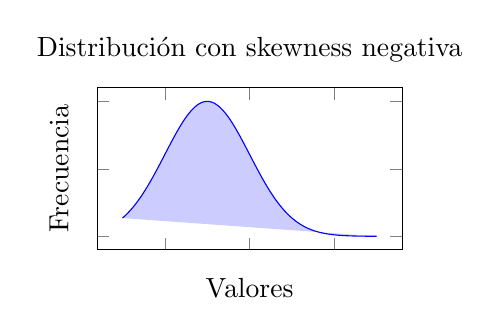
\begin{tikzpicture}
\begin{axis}[
    width=0.45\textwidth,
    height=0.3\textwidth,
    title={Distribución con skewness negativa},
    xlabel={Valores},
    ylabel={Frecuencia},
    yticklabels={,,},
    xticklabels={,,},
    domain=-3:3,
    samples=100,
    smooth,
    no markers
]
\addplot[fill=blue!20, draw=blue] {exp(-0.5*(x+1)^2)};
\end{axis}
\end{tikzpicture}
\hfill
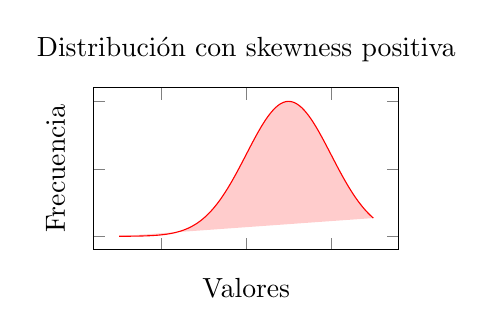
\begin{tikzpicture}
\begin{axis}[
    width=0.45\textwidth,
    height=0.3\textwidth,
    title={Distribución con skewness positiva},
    xlabel={Valores},
    ylabel={Frecuencia},
    yticklabels={,,},
    xticklabels={,,},
    domain=-3:3,
    samples=100,
    smooth,
    no markers
]
\addplot[fill=red!20, draw=red] {exp(-0.5*(x-1)^2)};
\end{axis}
\end{tikzpicture}
\caption{Ejemplos de distribuciones con skewness negativa (izquierda) y positiva (derecha)}
\label{fig:skewness}
\end{figure}
